\section{Tooling}\label{sec:tooling}

\subsection{ATM}\label{sec:atm}
ATM is a model-based testing web application, developed in the Ruby on Rails framework. It is used to test the software of several big companies in the Netherlands since 2006. It is under continuous development by Axini.

The architecture is shown graphically in Figure~\ref{fig:axini_tool}. It has a similar structure to the on-the-fly model-based testing tool architecture in Figure~\ref{fig:model_based_testing_on_the_fly}.

\begin{figure}[ht]
  \begin{center}
    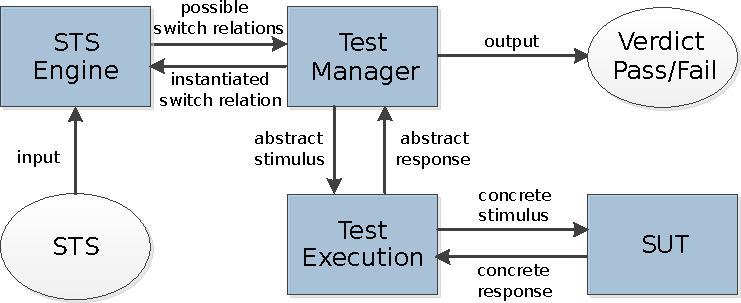
\includegraphics[width=0.75\textwidth]{axini_tool.pdf}
  \end{center}
  \caption{Architecture of ATM}
  \label{fig:axini_tool}
\end{figure}

The tool functions as follows: 
\begin{enumerate}
  \item An STS is given to an STS Engine, which keeps track of the current location and data values. It passes the possible switch relations from the current location to the Test Manager.
  \item The Test Manager chooses an enabled switch relation based on a test strategy, which can be a random strategy or a strategy designed to obtain a high location/switch relation coverage. The valuation of the variables in the guard are also chosen by a test strategy, which can be a random strategy or a strategy using boundary-value analysis. The choice is represented by an instantiated switch relation and passed back to the STS Engine, which updates its current location and data values. The communication between these two components is done by method calls.
  \item The gate of the instantiated switch relation is given to the Test Execution component as an \textit{abstract stimulus}. The term abstract indicates that the instantiated switch relation is an abstract representation of some computation steps taken in the SUT. For instance, a transition with label '?connect' is an abstract stimulus of the actual setup of a TCP connection between two distributed components of the SUT. 
  \item The translation of an abstract stimulus to a concrete stimulus is done by the Test Execution component. This component provides the stimulus to the SUT. When the SUT responds, the Test Execution component translates this response to an abstract response. For instance, the Test Execution component receives an HTTP response that the TCP connect was succesful. This is a concrete response, which the Test Execution component translates to an abstract response, such as a transition with label '!ok'. The Test Manager is notified with this abstract response.
  \item The Test Manager translates the abstract response to an instantiated switch relation and updates the STS Engine. If this is possible according to the model, the Test Manager gives a pass verdict for this test. Otherwise, the result is a fail verdict.
\end{enumerate}

\subsection{GROOVE}\label{sec:descriptiongroove}
GROOVE is an open source, graph-based modelling tool in development at the University of Twente since 2004~\cite{Rensink:GROOVE}. It has been applied to several case studies, such as model transformations and security and leader election protocols~\cite{Ghamarian:GROOVE}.

The architecture of the GROOVE tool is shown graphically in Figure~\ref{fig:groove_tool}. A graph grammar is given as input to the Rule Applier component, which determines the possible rule transitions. An Exploration Strategy can be started or the user can explore the states manually using the GUI. These components request the possible rule transitions and respond with the chosen rule transition (based on the exploration strategy or the user input). The Exploration Strategy can do an exhaustive search, resulting in a GTS. The graph states and rule transitions in this GTS can then be inspected using the GUI.

\begin{figure}[ht]
  \begin{center}
    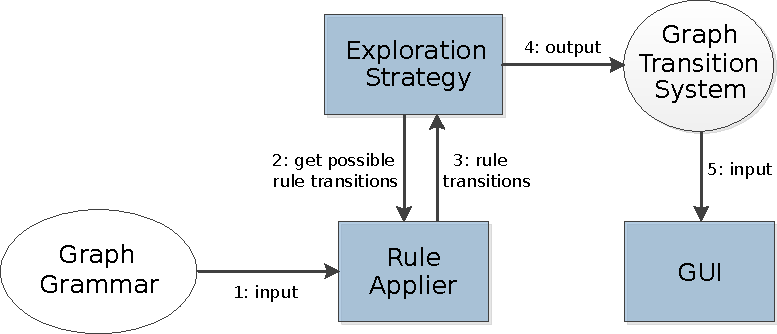
\includegraphics[width=0.75\textwidth]{groove_tool.pdf}
  \end{center}
  \caption{The GROOVE Tool}
  \label{fig:groove_tool}
\end{figure}

\subsection{Graph grammars in GROOVE}\label{sec:example_groove} 
The running example from Figure~\ref{fig:example_sts} is displayed as a graph grammar, as visualized in GROOVE, in Figure~\ref{fig:example_groove}. The $\mathit{LHS}$, $\mathit{RHS}$ and $\mathit{NAC}$ of a rule in GROOVE are visualized together in one graph. Figures~\ref{fig:example_groove_throw}, \ref{fig:example_groove_move} and \ref{fig:example_groove_next} show three rules. Figure~\ref{fig:example_groove_start} shows the start graph of the system.

\begin{figure}[ht]
  \begin{center}
    \subfloat[The start graph]{\label{fig:example_groove_start}% To use this figure in your LaTeX document
% import the package groove/resources/groove2tikz.sty
%
% Special colors
\begin{tikzpicture}[
% Special color styles
scale=\tikzscale]
\node[node] (n0)  at (2.250, -0.605) {\ml{\textbf{Die}\\rolls = 0}};
\node[node] (n10)  at (3.560, -2.025) {\ml{\textbf{Location}}};
\node[node] (n9)  at (0.930, -1.985) {\ml{\textbf{Location}}};
\node[node] (n8)  at (2.200, -2.545) {\ml{\textbf{Location}}};
\node[node] (n11)  at (0.990, -0.600) {\ml{\textbf{Player}\\\textit{turn}\\id = 1}};
\node[node] (n7)  at (2.180, -1.465) {\ml{\textbf{Location}}};
\node[node] (n12)  at (3.550, -0.615) {\ml{\textbf{Player}\\id = 2}};
\path[edge](n11.south -| 0.930, -1.985) -- node[lab]{at} (n9) ;
\path[edge] (n10)  -- node[lab]{next} (n8) ;
\path[edge] (n9)  -- node[lab]{next} (n7) ;
\path[edge] (n8)  -- node[lab]{next} (n9) ;
\path[edge] (n7)  -- node[lab]{next} (n10) ;
\path[edge](n12.south -| 3.560, -2.025) -- node[lab]{at} (n10) ;
\userdefinedmacro
\end{tikzpicture}
\renewcommand{\userdefinedmacro}{\relax}
}\quad
    \subfloat[The throw rule]{\label{fig:example_groove_throw}% To use this figure in your LaTeX document
% import the package groove/resources/groove2tikz.sty
%
% Special colors
\begin{tikzpicture}[
% Special color styles
scale=\tikzscale]
\node[node] (n1)  at (0.545, -0.470) {\ml{\textbf{Player}\\\textit{turn}}};
\node[node] (n5)  at (1.595, -1.295) {\ml{\textbf{Die}}};
\node[nacnode, attr] (n2)  at (0.495, -1.325) {\ml{\textbf{int}}};
\node[node, attr] (n4)  at (1.605, -0.405) {\ml{\textbf{int}}};
\node[parnode] (n4p)  at (n4.north west) {0};
\path[newedge](n1.east |- 1.605, -0.405) -- node[newlab]{throws} (n4) ;
\path[edge](n5.north -| 1.605, -0.405) -- node[lab]{canThrow} (n4) ;
\path[nacedge](n1.south -| 0.495, -1.325) -- node[naclab]{throws} (n2) ;
\userdefinedmacro
\end{tikzpicture}
\renewcommand{\userdefinedmacro}{\relax}
}
    \subfloat[The move rule]{\label{fig:example_groove_move}% To use this figure in your LaTeX document
% import the package groove/resources/groove2tikz.sty
%
% Special colors
\begin{tikzpicture}[
% Special color styles
scale=\tikzscale]
\node[node] (n3)  at (2.840, -0.970) {\ml{\textbf{Die}\\{\color{\green}rolls := rolls $-$ 1}\\rolls $\>$ 0}};
\node[node] (n1)  at (1.540, -1.925) {\ml{\textbf{Location}}};
\node[node] (n0)  at (1.460, -0.970) {\ml{\textbf{Player}\\\textit{turn}}};
\node[node] (n2)  at (2.760, -1.915) {\ml{\textbf{Location}}};
\node[node, attr] (n4)  at (1.480, -0.400) {\ml{\textbf{int}}};
\node[parnode] (n4p)  at (n4.north west) {0};
\path[newedge] (n0)  -- node[newlab]{at} (n2) ;
\path[deledge](n0.south -| 1.540, -1.925) -- node[dellab]{at} (n1) ;
\path[edge](n1.east |- 2.760, -1.915) -- node[lab]{next} (n2) ;
\path[edge](n0.east |- 2.840, -0.970) -- node[lab]{throws} (n3) ;
\path[edge](n0.north -| 1.480, -0.400) -- node[lab]{id} (n4) ;
\userdefinedmacro
\end{tikzpicture}
\renewcommand{\userdefinedmacro}{\relax}
}
    \subfloat[The next turn rule]{\label{fig:example_groove_next}% To use this figure in your LaTeX document
% import the package groove/resources/groove2tikz.sty
%
% Special colors
\begin{tikzpicture}[
% Special color styles
scale=\tikzscale]
\node[node] (n0)  at (1.090, -0.650) {\ml{\textbf{Player}\\{\color{\blue}\textit{$-$ turn}}}};
\node[node] (n2)  at (2.050, -0.660) {\ml{\textbf{Player}\\{\color{\green}\textit{$+$ turn}}}};
\node[node] (n3)  at (1.080, -1.730) {\ml{\textbf{Die}\\rolls = 0}};
\path[edge, -](n0.east |- 2.050, -0.660) -- node[lab]{\textit{!=}} (n2) ;
\path[deledge](n0.south -| 1.080, -1.730) -- node[dellab]{throws} (n3) ;
\userdefinedmacro
\end{tikzpicture}
\renewcommand{\userdefinedmacro}{\relax}
}
  \end{center}
  \caption{The graph grammar of the board game example in Figure~\ref{fig:example_sts}}
  \label{fig:example_groove}
\end{figure}

The colors on the nodes and edges in the rules represent whether they belong to the $\mathit{LHS}$, $\mathit{RHS}$ or $\mathit{NAC}$ of the rule.
\begin{enumerate}
  \item normal line (black): This node or edge is part of both the $\mathit{LHS}$ and $\mathit{RHS}$.
  \item dotted line (red): This node or edge is part of the $\mathit{NAC}$ only.
  \item thick line (green): This node or edge is part of the $\mathit{RHS}$ only.
  \item dashed line (blue): This node or edge is part of the $\mathit{LHS}$ only.
\end{enumerate}

The rules can be described as follows:
\begin{enumerate}
  \item~\ref{fig:example_groove_throw}: 'if a player has the turn and he has not thrown the die yet, he may do so.'
  \item~\ref{fig:example_groove_move}: 'if a player has the turn and he has thrown the die and this number is larger than zero, he may move one place and then it is as if he has thrown one less.'
  \item~\ref{fig:example_groove_next}: 'if a player has finished moving (number thrown is zero), the next player receives the turn.'
\end{enumerate}

The strings on the nodes are a short-hand notation. The bold strings, \textbf{Die}, \textbf{Player}, \textbf{Location} and \textbf{int} indicate the \textit{type} of the node. Nodes with a type starting with a lower case letter, such as \textbf{int}, are variable nodes from $\mathcal{V}$. The italic string \textit{turn}, is a representation of a self-edge with label $turn$. In the next turn rule, the $turn$ edge exists in the $\mathit{LHS}$ as a self-edge of the left \textbf{Player} node and in the $\mathit{RHS}$ as a self-edge of the right \textbf{Player} node. In the same rule, the $throws$ edge from the left \textbf{Player} node to an integer node only exists in the $\mathit{LHS}$.

The assignments on the \textbf{Die} node are representations of edges labelled 'canThrow' to variable nodes. The six variable nodes are of the type integer and each have an initial value of one to six. The throws value assignment (:=) in the move rule is a shorthand for two edges: one edge in the $\mathit{LHS}$ with label $throws$ from the \textbf{Player} node to an integer node with value $i$ and another edge in the $\mathit{RHS}$ with label $throws$ from the \textbf{Player} node to an integer node with value $i-1$. 

The 'throws > 0' is a term over the variable node that is the target of an outgoing edge labeled 'throws'. In this case, the valuation of the term be true for the rule to match the graph.

The number '0' in the top left of the \textbf{int} node in the throw rule indicates that this integer is the first parameter in $param(l)$, where $l$ is the label on the rule transition created by applying the throws rule.

The graph is transformed after the rule is applied. The resulting graph after the transformation is the new state of the system and the rule is the transition from the old state (the graph as it was before the rule was applied) to the new state. Figure~\ref{fig:gts_example} shows the IOGTS of one \textit{?throws} rule application on the start graph. Note that the \textit{?throws} is an input, as indicated by the '?'. State $s_1$ is a representation of the graph in Figure~\ref{fig:example_groove_start}. Figure~\ref{fig:target_graph_state} shows the graph represented by $s_2$.

\begin{figure}[ht]
  \begin{center}
    % To use this figure in your LaTeX document
% import the package groove/resources/groove2tikz.sty
%
% Special colors
\begin{tikzpicture}[
% Special color styles
scale=\tikzscale]
\node[node, start] (s0)  at (0.560, -0.155) {\ml{\textit{s0}}};
\node[node, open, bold] (s1)  at (0.565, -0.865) {\ml{\textit{s1}}};
\path[edge](s0.south -| 0.565, -0.865) -- node[lab]{throws?(2)} (s1) ;
\userdefinedmacro
\end{tikzpicture}
\renewcommand{\userdefinedmacro}{\relax}

  \end{center}
  \caption{The GTS after one rule application on the board game example in Figure~\ref{fig:example_groove}}
  \label{fig:gts_example}
\end{figure}

\begin{figure}[ht]
  \begin{center}
    % To use this figure in your LaTeX document
% import the package groove/resources/groove2tikz.sty
%
% Special colors
\begin{tikzpicture}[
% Special color styles
scale=\tikzscale]
\node[node] (n12)  at (5.615, -0.525) {\ml{\textbf{Player}}};
\node[node] (n7)  at (4.245, -1.375) {\ml{\textbf{Location}}};
\node[node] (n11)  at (3.055, -0.520) {\ml{\textbf{Player}\\\textit{turn}\\throws = 2}};
\node[node] (n8)  at (4.265, -2.455) {\ml{\textbf{Location}}};
\node[node] (n9)  at (2.995, -1.895) {\ml{\textbf{Location}}};
\node[node] (n10)  at (5.625, -1.935) {\ml{\textbf{Location}}};
\node[node] (n0)  at (1.585, -0.865) {\ml{\textbf{Die}\\canThrow = 1\\canThrow = 2\\canThrow = 3\\canThrow = 4\\canThrow = 5\\canThrow = 6}};
\path[edge] (n8)  -- node[lab]{next} (n9) ;
\path[edge](n12.south -| 5.625, -1.935) -- node[lab]{at} (n10) ;
\path[edge] (n7)  -- node[lab]{next} (n10) ;
\path[edge](n11.south -| 2.995, -1.895) -- node[lab]{at} (n9) ;
\path[edge] (n9)  -- node[lab]{next} (n7) ;
\path[edge] (n10)  -- node[lab]{next} (n8) ;
\userdefinedmacro
\end{tikzpicture}
\renewcommand{\userdefinedmacro}{\relax}

  \end{center}
  \caption{The graph of state $s2$ in Figure~\ref{fig:gts_example}}
  \label{fig:target_graph_state}
\end{figure}
